\chapter{Alta disponibilidade}
\label{cap:altadiponibilidade}

Alta disponibilidade é um termo muito conhecido, sendo cada vez mais empregada nos ambientes computacionais. O objetivo de promover 
alta disponibilidade resume-se em garantir que um serviço esteja sempre disponível quando o cliente solicitar ou acessar \cite{costa2009}.
A alta disponibilidade é definida como a redundância de \textit{hardware} ou de \textit{software} para que o serviço fique mais tempo disponível.
Quanto maior for a disponibilidade desejada maior deverá ser a redundância no ambiente, assim reduzindo os pontos únicos de falha,
que em inglês são chamados de \ac{SPOF}. A alta disponibilidade está diretamente relacionada a: 
\begin{itemize}
 \item Dependabilidade: indica a qualidade do serviço fornecido e a confiança depositada neste serviço. A dependabilidade envolve atributos 
 como segurança de funcionamento, segurança de acesso, manutenabilidade, testabilidade e comprometimento do desempenho \cite{weber2002};
 \item Confiabilidade: é o atributo mais importante, pois transmite a ideia de continuidade de serviço \cite{pankaj1994}. A confiabilidade 
 refere-se a probabilidade de um serviço funcionar corretamente durante um dado intervalo de tempo;
 \item Disponibilidade: é a probabilidade de um serviço estar operacional no instante em que for solicitado \cite{costa2009};
 \item Tolerância a falhas: procura garantir a disponibilidade de um serviço utilizando mecanismos capazes de detectar, mascarar e recuperar 
 falhas, e seu objetivo é alcançar a dependabilidade, assim indicando uma boa qualidade de serviço \cite{costa2009}. A tolerância a falhas é 
 um dos principais conceitos da alta diponibilidade, sendo assim será melhor discutida na Seção \ref{section:toleranciafalhas}.
\end{itemize}

\section{Tolerância a falhas}
\label{section:toleranciafalhas}

Sabe-se que o \textit{hardware} tende a falhar, principalmente devido a fatores físicos, por isso utiliza-se métodos para a prevenção 
de falhas e para a tolerância a falhas. A abordagem prevenção de falhas defini-se como um projeto feito na criação de componentes para
impedir que futuras falhas ocorram. Além disso, a prevenção de falhas melhora a disponibilidade e a confiabilidade de um serviço, isto é, 
tem como objetivo prever e eliminar o maior número de falhas possíveis antes de colocar o sistema em uso. Mas essa prevenção não resolverá 
todas as possíveis falhas. Sendo assim, a tolerância a falhas fornece disponibilidade de um serviço mesmo com a presença de falhas. 
Enquanto a prevenção de falhas tem foco nas fases de projeto, teste e validação, a tolerância a falhas tem como foco na utilização de 
componentes replicados para mascarar as falhas \cite{pankaj1994}.

O objetivo da tolerância a falhas é aumentar a disponibilidade de um sistema, isto é, aumentar o tempo que os serviços fornecidos aos 
clientes ou usuários ficam disponíveis. Um sistema é dito tolerante a falhas se ele pode mascarar a presença de falhas ou recuperar-se 
de uma falha. A tolerância a falhas é implementada utilizando redundância, que será detalhada na Seção \ref{section:redundancia}. 
Um exemplo frequentemente utilizando hoje em dia é tolerância a falhas em servidores de virtualização MELHOR EXEMPLO ???, onde normalmente
existem dois servidores com os seus dados replicados. Caso um dos servidores falhe por algum motivo, um \textit{software} de monitoramento
fará a transferência das maquinas virtuais para o outro servidor evitando assim a indisponibilidade do serviço. Este tema, virtualização, 
será detalhado no Capítulo \ref{cap:virtualizacao}.

A tolerância a falhas pode ser dividida em dois tipos que são: mascaramento; ou detecção, localização e reconfiguração.
O primeiro tipo, o mascaramento, não se manifesta na forma de erro sendo assim não necessita que o sistema trate este erro,
pois as falhas são tratadas na origem. O mascaramento é utilizado principalmente em sistemas de tempo real crítico. 
Um exemplo são os códigos de correção de erros, em inglês \ac{ECC}, que são utilizados em memórias para detecção e correção de erros.
No segundo tipo consiste em detectar, localizar e reconfigurar o \textit{software} ou \textit{hardware} e por fim resolver a 
falha \cite{weber2002}. O último tipo será melhor detalhado na Seção \ref{section:fasestolerancia}.

\subsection{Fases da tolerância a falhas}
\label{section:fasestolerancia}

A classificação das fases de tolerância a falhas mais comuns são detecção, confinamento, recuperação e tratamento \cite{weber2002}.

%\begin{figure}[falhasrecup]
% \centering
% 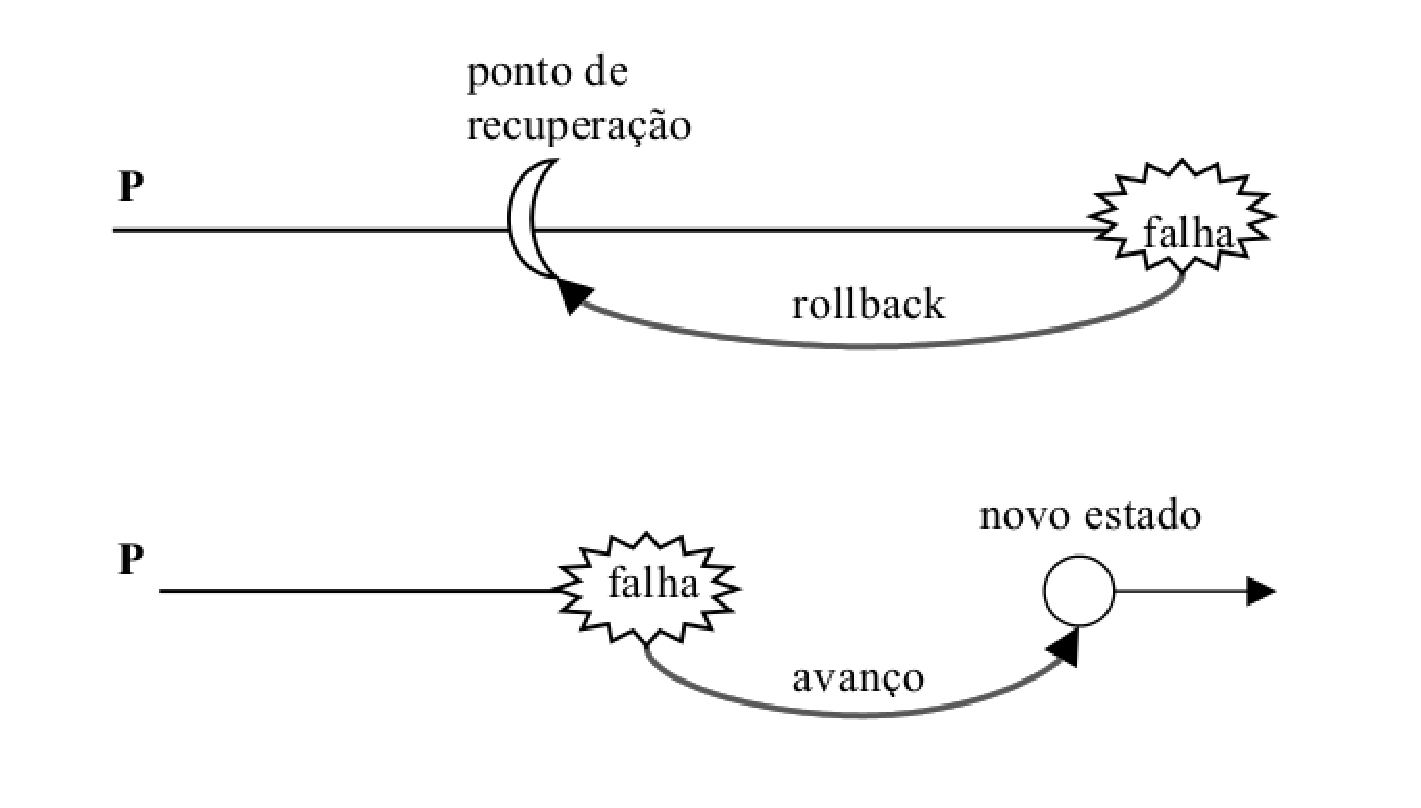
\includegraphics[height=200px]{img/recuperacao_ret_ava.eps}
% \caption{Recuperação por retorno e por avanço.}
% \label{fig:recuperacao_ret_ava}
%\end{figure}
% exemplo referencia: \ref{fig:recuperacao_ret_ava}

\begin{itemize}
 \item Detecção: realiza o monitoramento e aguarda uma falha se manifestar na forma de erro, para então passar para a próxima fase. 
 Um exemplo de detecção de erro é o cão de guarda (\textit{watchdog timer}), que recebe um sinal do programa ou serviço que esta sendo 
 monitorado e caso este sinal não seja recebido, devido alguma falha, o \textit{watchdog} irá se manifestar na forma de erro. 
 Outro exemplo é o esquema de duplicação e comparação, onde é feito operações em componentes replicados com mesmos dados de entrada, e então
 seus dados de saída são comparados, assim se houver alguma diferença um erro é gerado.
 \item Confinamento: responsável pela restrição de um erro para que esse não se propague para todo o sistema, pois entre a falha e a
 detecção do erro há um intervalo de tempo. Neste intervalo pode ocorrer a propagação do erro para outros componentes do sistema, sendo assim 
 antes de executar medidas corretivas é necessário definir os limites da propagação. EXEMPLO ???
 \item Recuperação: após a detecção de um erro ocorre a recuperação, onde o estado de erro é alterado para estado livre de erros. A recuperação
 pode ser feita de duas formas, que são:
 \begin{itemize}
  \item \textit{forward error recovery} (recuperação por avanço): ocorre uma condução para um novo estado não ocorrido anteriormente. É a forma
  de recuperação mais eficiente, porém mais complexo de ser implementado pois a ação deve ser precisa.
  \item \textit{backward error recovery} (recuperação por retorno): ocorre um retorno para um estado anterior que deve estar livre de erros.
  Para retornar ao estado anterior pode ser utilizado pontos de recuperação (\textit{checkpoints}), e quando ocorrer um erro, um \textit{rollback} 
  é executado, ou seja, retornará a um estado anterior a falha.
 \end{itemize}
 \item Tratamento: procura prevenir que futuros erros aconteçam. Nesta fase ocorre a localização da falha para descobrir o 
 componente que originou a falha. A substituição do componente danificado pode ser feita de duas formas, manual ou automática. 
 O reparo manual é feito por um operador, e o automático quando existe um componente em espera para substituição. Exemplo de um reparo 
 manual é um operador que efetua a troca de um disco de um servidor. E um exemplo de reparo automático é um disco configurado como 
 \textit{hot spare}, ou seja, um componente de \textit{backup} que assumirá o lugar do outro imediatamente após o componente principal 
 falhar. Em \textit{storages} ou servidores o \textit{hot spare} pode ser configurado através de um \ac{RAID} \cite{rouse2013}.
\end{itemize}

\section{Redundância}
\label{section:redundancia}

Redundância pode ser feita através da replicação de componentes, para reduzir o número de \ac{SPOF} e garantir o mascaramento de falhas.
Na prática, se um componente falhar ele deve ser reparado ou substituído por um novo, sem que haja uma interrupção no serviço.
A redundância pode ser implementada ainda através do envio de sinais ou \textit{bits} de controle junto aos dados, servindo assim para 
detecção de erros e até para correção \cite{weber2002}. Segundo \cite{norvag2000} existem quatro tipos diferentes de redundância que são:
\begin{itemize}
 \item \textit{Hardware}: utiliza-se a replicação de componentes, sendo que caso um falhe outro possa assumir seu lugar. 
 Para fazer a detecção de erros a saída de cada componente é constantemente monitorada e comparada à saída de outros componentes.
 Um exemplo prático de redundância de \textit{hardware} são os servidores com fontes redundantes. Nestes são utilizadas duas fontes ligadas 
 em paralelo, sendo que caso uma falhe a outra suprirá a necessidade de todo o servidor;
 \item Informação: ocorre quando uma informação extra é enviada ou armazenada para possibilitar a detecção e correção de erros.
 Um exemplo clássico são os \textit{checksums} (soma de verificação). Esses são calculados antes da transmissão ou armazenamento dos dados 
 e recalculado ao recebê-los ou recuperá-los, assim sendo possível verificar a integridade dos dados. Outro exemplo bastante comum são os 
 \textit{bits} de paridade que são utilizandos para detectar falhas que afetam apenas um \textit{bit} \cite{weber2002};
 \item \textit{Software}: CONCEITO EXEMPLO MYSQL REPLICACAO ???. 
 Outro maneira de implementar redundância de \textit{software} é através da replicação do mesmo \textit{software}, que não é muito útil 
 pois replicando um \textit{software} as falhas ou \textit{bugs} estarão presentes em todas replicas. Existem algumas técnicas que podem 
 ajudar com esse problema. A programação de \textit{n}-versões é uma delas, que consiste em criar \textit{n} versões para um mesmo 
 \textit{software}. Desta forma, possibilita-se o aumento da disponibilidade, uma vez que elas provavelmente não apresentarão os mesmos 
 erros. Por outro lado a programação de \textit{n}-versões possui um custo muito elevado devido a complexidade da sua manutenção.
 \item Tempo: este é feito através da execução de um conjunto de instruções várias vezes no mesmo componente, assim detectando uma falha caso 
 ocorra. Essa técnica necessita tempo adicional, e é utilizada onde o tempo não é crítico. Por exemplo, um \textit{software} de monitoramento 
 de serviços e servidores, que faz um teste em cada serviço e caso ocorra uma falha o \textit{software} poderá executar uma ação corretiva para 
 reestabelecer o serviço. Essa técnica, diferentemente da redundância de \textit{hardware} e informação, não requer um \textit{hardware} 
 extra para sua implementação \cite{costa2009}.
\end{itemize}

\section{Cálculo da alta disponibilidade}

Um ponto importante sobre alta diponibilidade é como medi-la. Para isso são utilizados os valores de \textit{uptime} e \textit{downtime}, 
que são respectivamente, o tempo que os serviços estão funcionando normalmente e o tempo que não estão funcionando. A alta disponibilidade 
pode ser expressa pela quantidade de ``noves'', isto é, se um serviço possui quatro noves de disponibilidade, este possui uma 
disponibilidade de 99,99\% \cite{pereirafilho2004}.

\begin{table}
\caption {Níveis de alta disponibilidade e exemplos de sistemas}
\label{tab:dispniveis}
\begin{center}
\begin{tabular}{|l|l|l|l|}\hline
Nível & Uptime & Downtime por ano & Exemplos\\\hline
1 & 90\% & 36.5 dias & computadores pessoais\\\hline
2 & 98\% & 7.3 dias & \\\hline
3 & 99\% & 3.65 dias & sistemas de acesso\\\hline
4 & 99.8\% & 17 horas e 30 minutos & \\\hline
5 & 99.9\% & 8 horas e 45 minutos & provedores de acesso\\\hline
6 & 99.99\% & 52.5 minutos & CPD, sistemas de negócios\\\hline
7 & 99.999\% & 5.25 minutos & sistemas de telefonia ou bancários\\\hline
8 & 99.9999\% & 31.5 minutos & sistemas de defesa militar\\\hline
\end{tabular}
\end{center}
\end{table}

A Tabela \ref{tab:dispniveis} apresenta alguns níveis de disponibilidade, a sua porcentagem do \textit{Uptime}, o \textit{Downtime} por ano 
e a última coluna possui alguns exemplos de serviços relacionados ao nível de disponibilidade. Pode-se observar que para alguns serviços, 
como por exemplo sistemas bancários ou sistemas militares é necessário um alto nível de disponibilidade.

A porcentagem de diponibilidade pode ser calculada através da equação
\begin{equation}
d = \frac{MTBF}{(MTBF + MTTR)}
\label{diponibilidade}
\end{equation}
onde \ac{MTBF} é o tempo médio entre falhas, ou seja, esse corresponde ao tempo médio entre as paradas de um serviço. Já o \ac{MTTR} é o 
tempo médio de recuperação, isto é, o tempo entre a queda e a recuperação de um serviço \cite{goncalves2009}.

A alta disponibilidade é um dos principais fatores que fornece confiança aos clientes ou usuários, sendo extremante importante 
em empresas que fornecem serviços \textit{on-line}. Por isso existe o \ac{SLA}, que é um acordo de nível de serviço, que garante que 
o serviço fornecido atenda as expectativas dos clientes. Um \ac{SLA} é um documento contendo uma descrição e uma definição das 
características mais importantes do serviço que será fornecido. Esse acordo também deve conter o nível de serviço exigido pelo negócio, 
isto é, a porcentagem da diponibilidade exigida, sendo que esta deve ser minuciosamente definido. Por exemplo, um \ac{SLA} pode conter 
descrição do serviço, requerimentos, horário de funcionamento, entre outros \cite{smith2010}.
